\documentclass[11pt,letterpaper]{article}
\usepackage[margin=1in]{geometry}
\usepackage[english]{babel}
\usepackage[utf8x]{inputenc}
\usepackage{amsmath}
\usepackage{amssymb} 
\usepackage{graphicx}
\usepackage{tabularx}
\usepackage{epstopdf}
\usepackage{subfig}
\usepackage{bbm}
\usepackage{kpfonts}    % for nice fonts
\usepackage{microtype} 
\usepackage{booktabs}   % for nice tables
\usepackage{bm}         % for bold math
\usepackage{listings}   % for inserting code
\usepackage{verbatim}   % useful for program listings
\usepackage{color}  
\usepackage[colorlinks=true]{hyperref}
\usepackage{setspace}
% use for hypertext

\usepackage{natbib}
\usepackage{authblk}
\usepackage[hang,flushmargin,multiple]{footmisc} %dont indent footnotes
\newcommand{\hilight}[1]{\colorbox{yellow}{#1}}
\hypersetup{colorlinks=true,linkcolor=black,citecolor=black,urlcolor=black}

\newcolumntype{K}[1]{>{\centering\arraybackslash}p{#1}}



\title{Benefits in a SNAP: The Effects of the Online Application for Food Stamps}
\author[1]{Andrew Foote}
\author[2]{Michel Grosz}
\author[3]{Stephanie Rennane}
\author[4]{Somebody Else}
\affil[1]{Census Bureau}
\affil[2]{Abt Associates}
\affil[3]{RAND Corporation}
\date{\today\\  }





\begin{document}
\maketitle

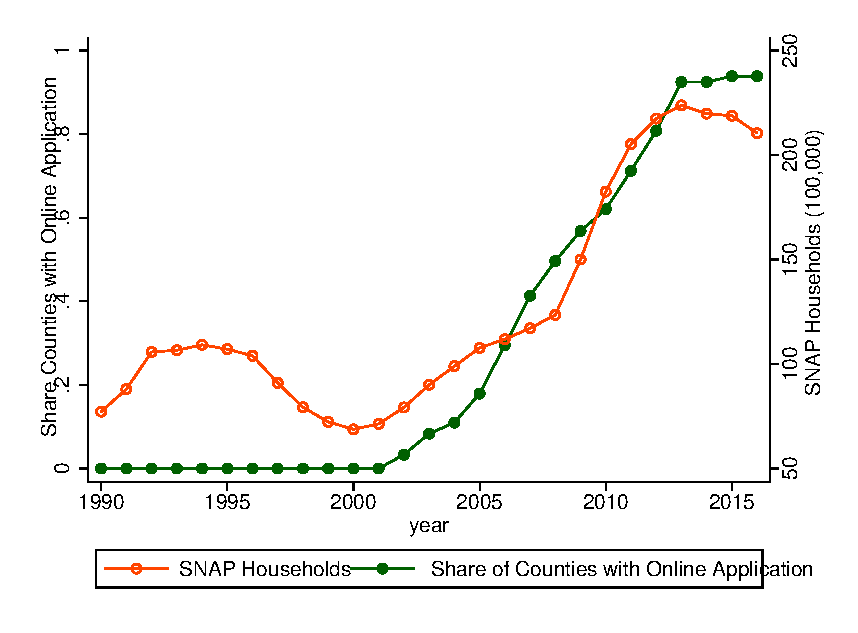
\includegraphics{tabfig/rolloutgraph_share}

%\begin{table}\caption{Main Effects of Post-Adoption on ln(beneficiaries)}
%\def\sym#1{\ifmmode^{#1}\else\(^{#1}\)\fi}
%\begin{tabular}{lcccc}\hline\hline
%A. All Counties\\\input{ddreg_pu_all}\\
%B. Adopting Counties\\\input{ddreg_pu_adop}\\
%C. All Counties, ln(+1)\\\input{ddreg_in0_all}\\
%D. Adopting Counties, ln(+1)\\\input{ddreg_in0_adop}\\
%Year FE&&X&X&X\\
%State FE&&&X&X\\
%County Trends&&&&X\\
%\hline\hline
%\end{tabular}
%\end{table}



\begin{figure}\caption{Event Study Estimates, BEA count}
\begin{tabular}{cc}
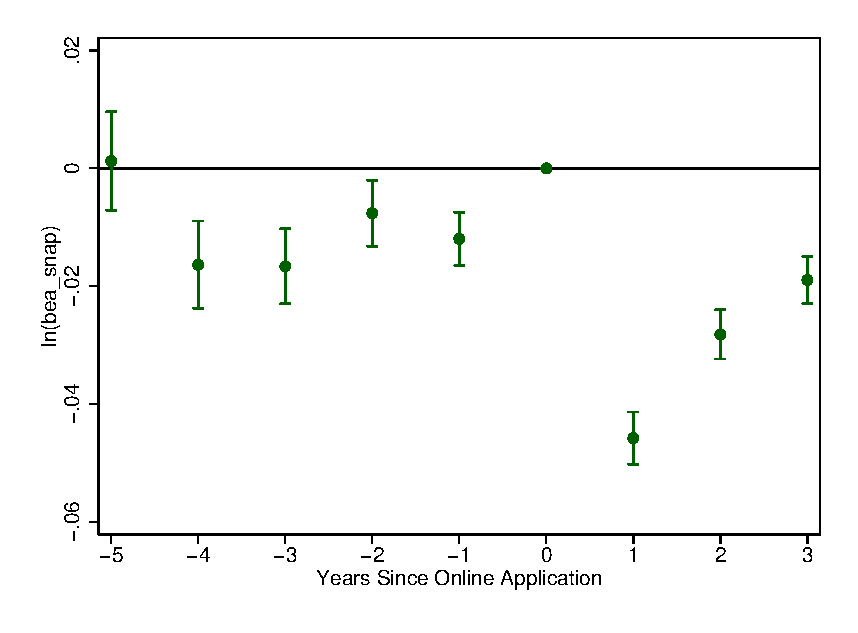
\includegraphics[scale=0.57]{tabfig/evstu_bea_snap_one_yrcf_5_3}&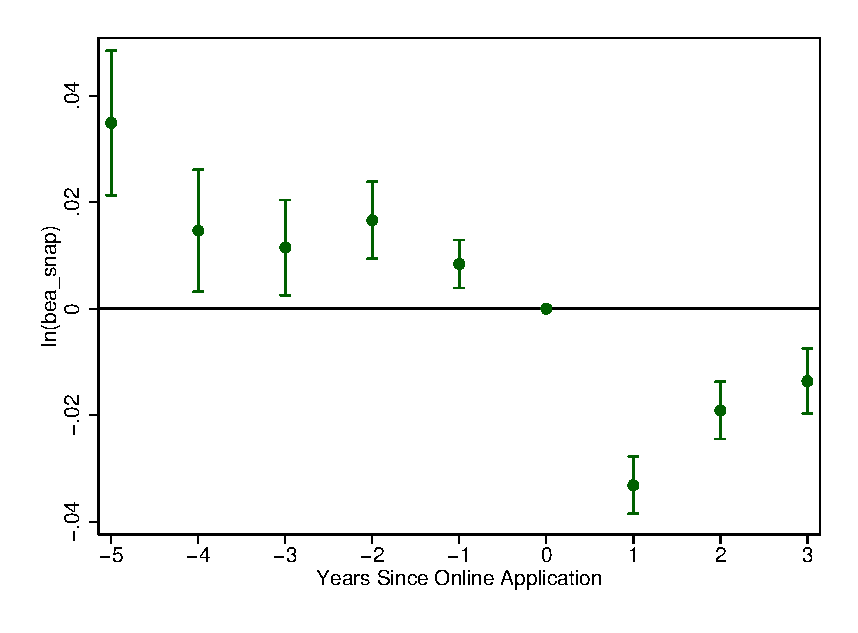
\includegraphics[scale=0.57]{tabfig/evstu_bea_snap_one_yrcfsttr_5_3}\\
a) Year FE and County FE&b) Year FE, County FE+Trends\\
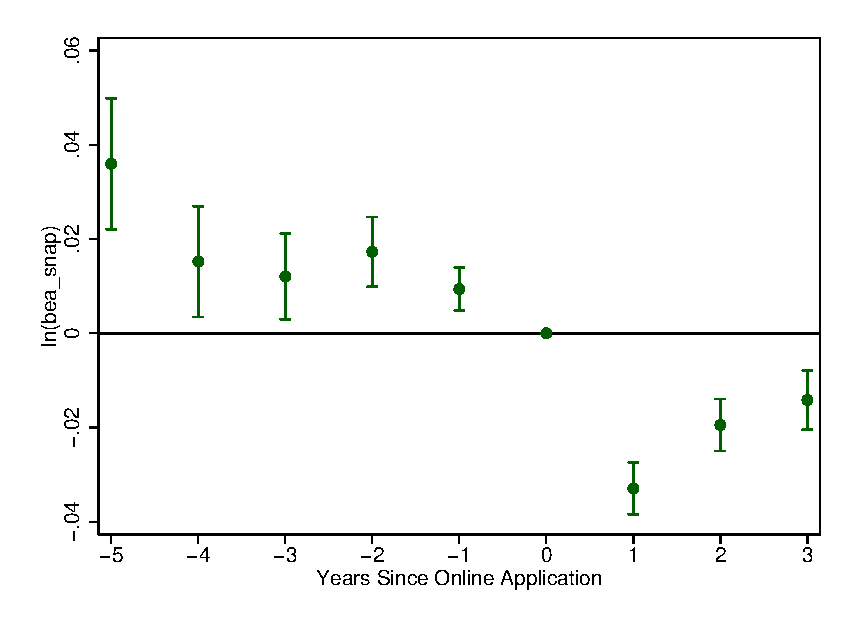
\includegraphics[scale=0.57]{tabfig/evstu_bea_snap_one_yrcfcttru_5_3}&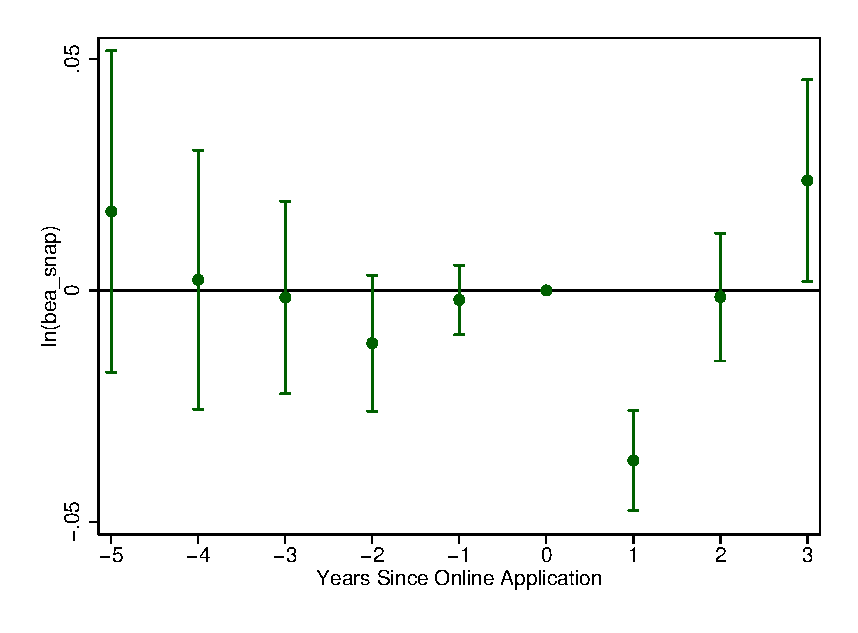
\includegraphics[scale=0.57]{tabfig/evstu_bea_snap_total_pop_yrcfcttru_5_3}\\
c) Year FE, County FE+Trends, UI control& c) Year FE, County FE + Trends, UI control, weighted\\
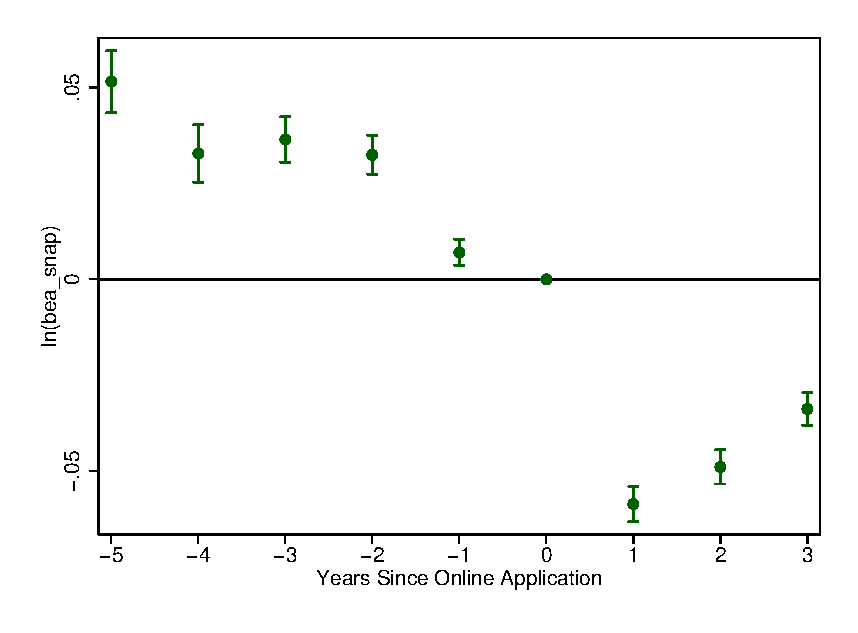
\includegraphics[scale=0.57]{tabfig/evstu_bea_snap_one_yrcfcttrunor_5_3}\\
e) Year FE, County FE + Trends, UI control, no Recession\\
\end{tabular}
\end{figure}

\begin{figure}\caption{Event Study Estimates, Households}
\begin{tabular}{cc}
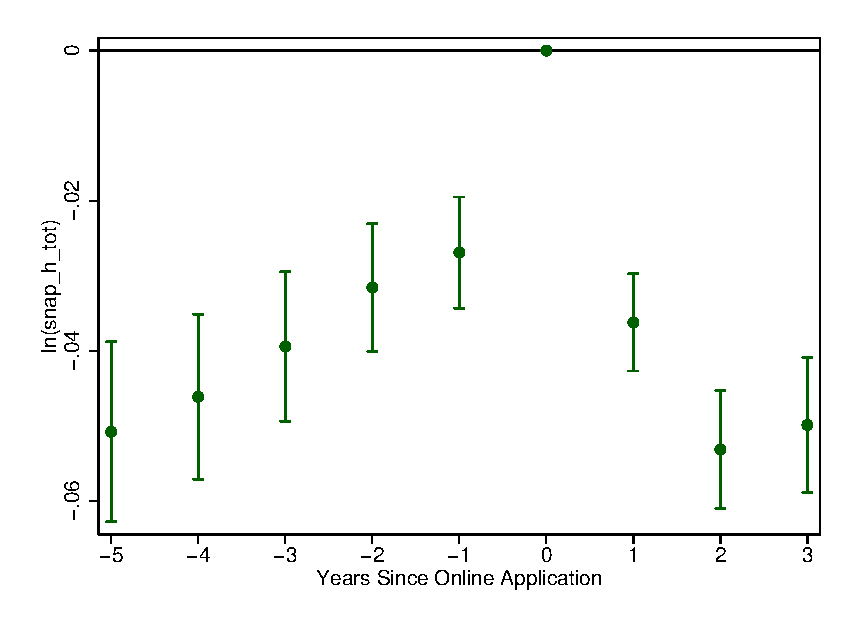
\includegraphics[scale=0.57]{tabfig/evstu_snap_h_tot_one_yrcf_5_3}&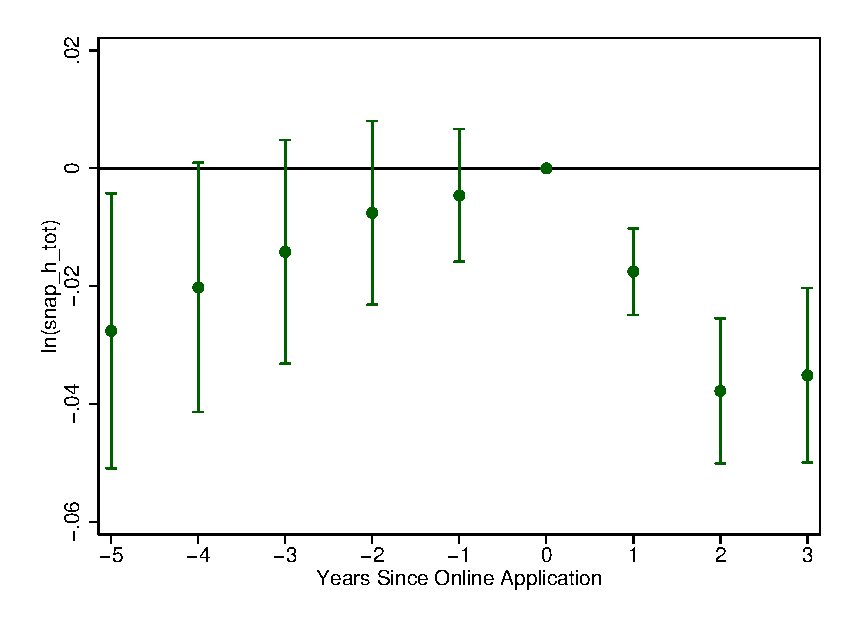
\includegraphics[scale=0.57]{tabfig/evstu_snap_h_tot_one_yrcfsttr_5_3}\\
a) Year FE and County FE&b) Year FE, County FE+Trends\\
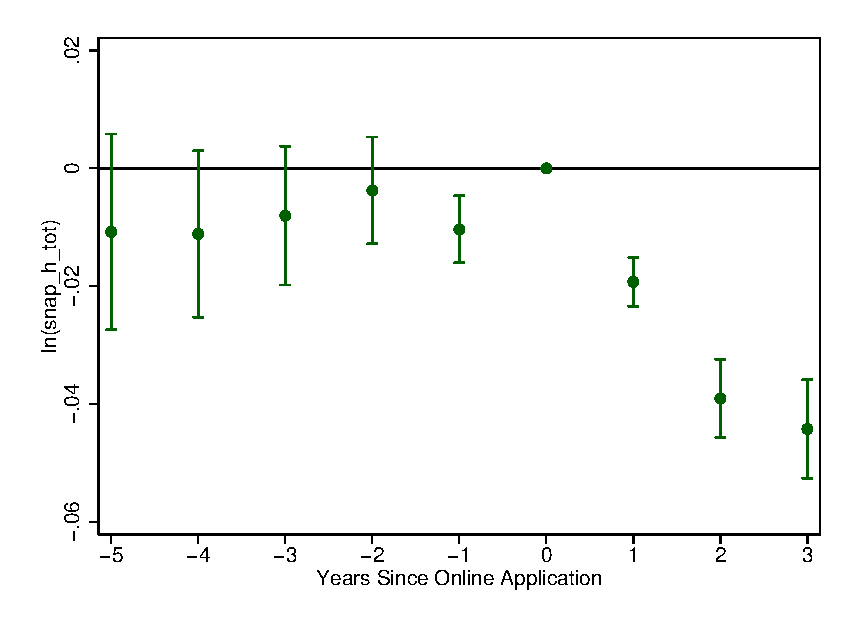
\includegraphics[scale=0.57]{tabfig/evstu_snap_h_tot_one_yrcfcttru_5_3}&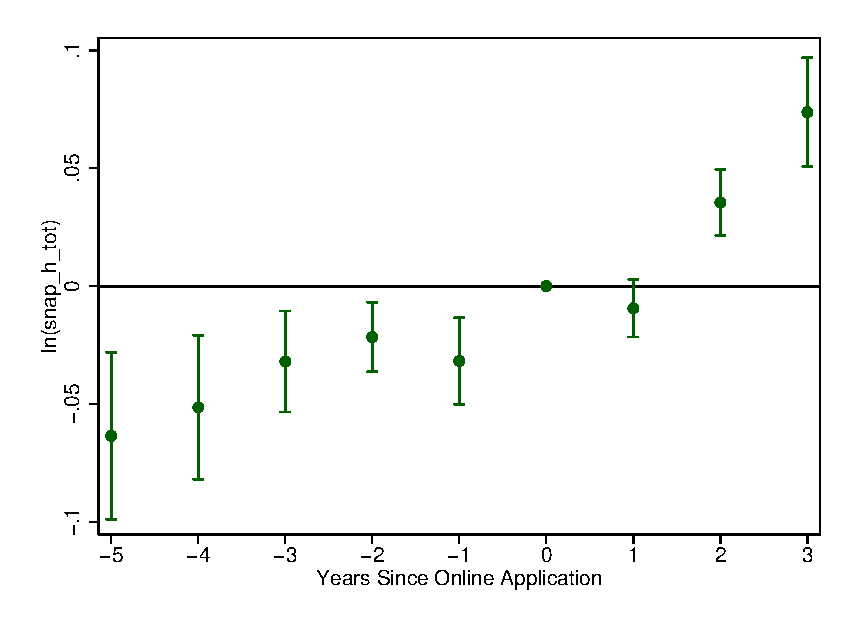
\includegraphics[scale=0.57]{tabfig/evstu_snap_h_tot_total_pop_yrcfcttru_5_3}\\
c) Year FE, County FE+Trends, UI control& c) Year FE, County FE + Trends, UI control, weighted\\
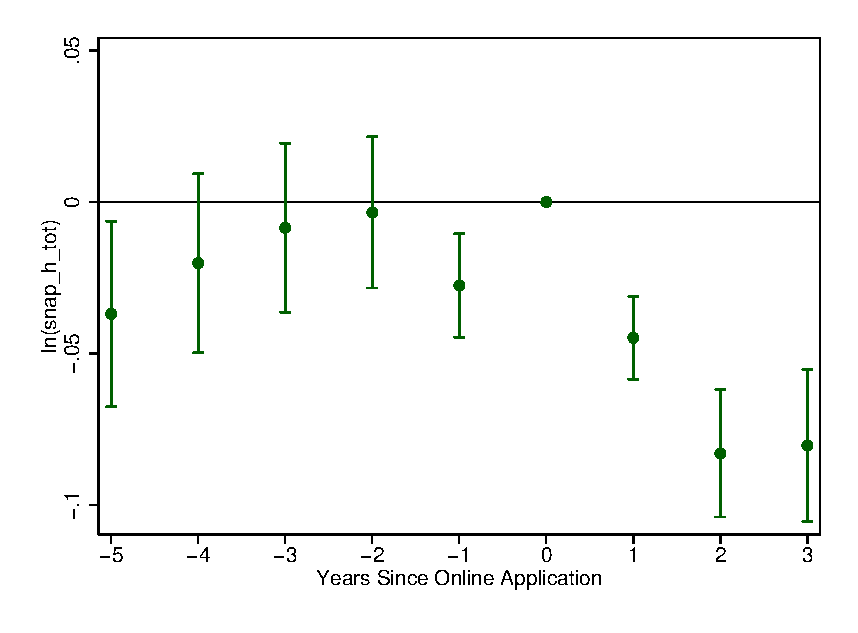
\includegraphics[scale=0.57]{tabfig/evstu_snap_h_tot_one_yrcfcttrunor_5_3}\\
e) Year FE, County FE + Trends, UI control, no Recession\\
\end{tabular}
\end{figure}


\begin{figure}\caption{Event Study Estimates, Individuals}
\begin{tabular}{cc}
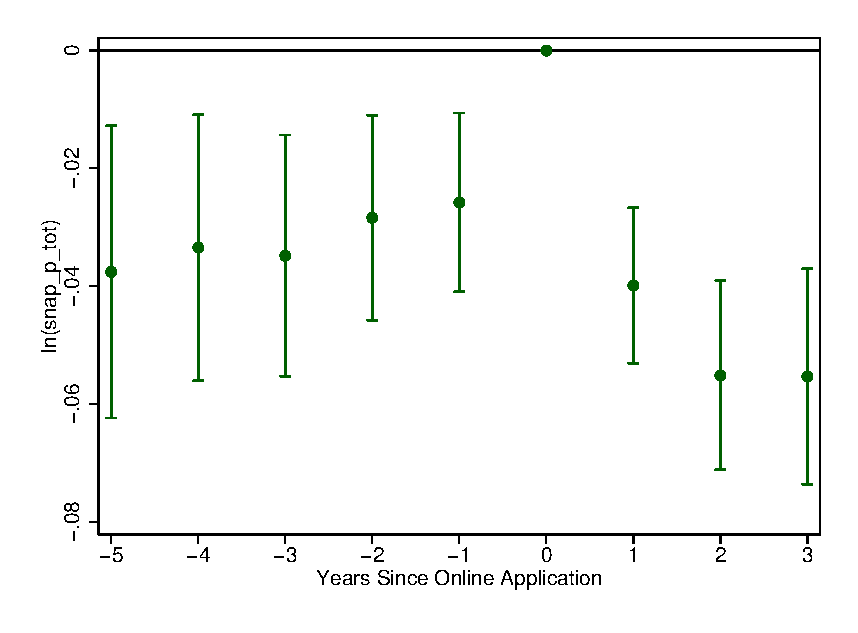
\includegraphics[scale=0.57]{tabfig/evstu_snap_p_tot_one_yrcf_5_3}&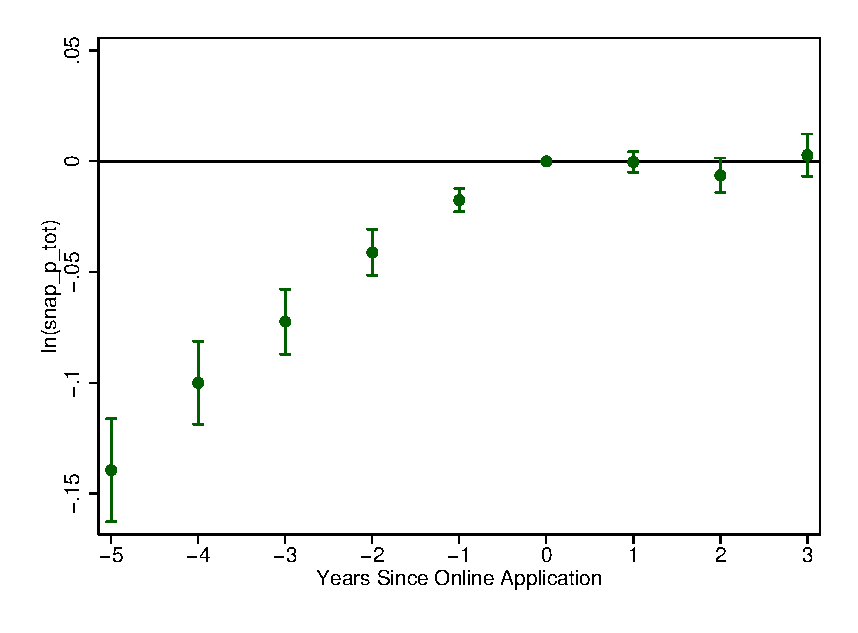
\includegraphics[scale=0.57]{tabfig/evstu_snap_p_tot_one_yrcfsttr_5_3}\\
a) Year FE and County FE&b) Year FE, County FE+Trends\\
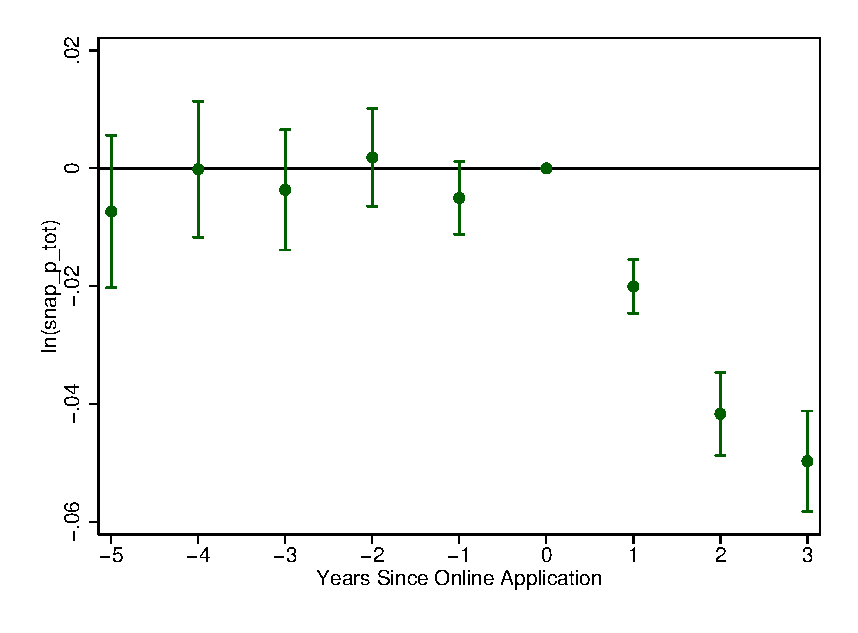
\includegraphics[scale=0.57]{tabfig/evstu_snap_p_tot_one_yrcfcttru_5_3}&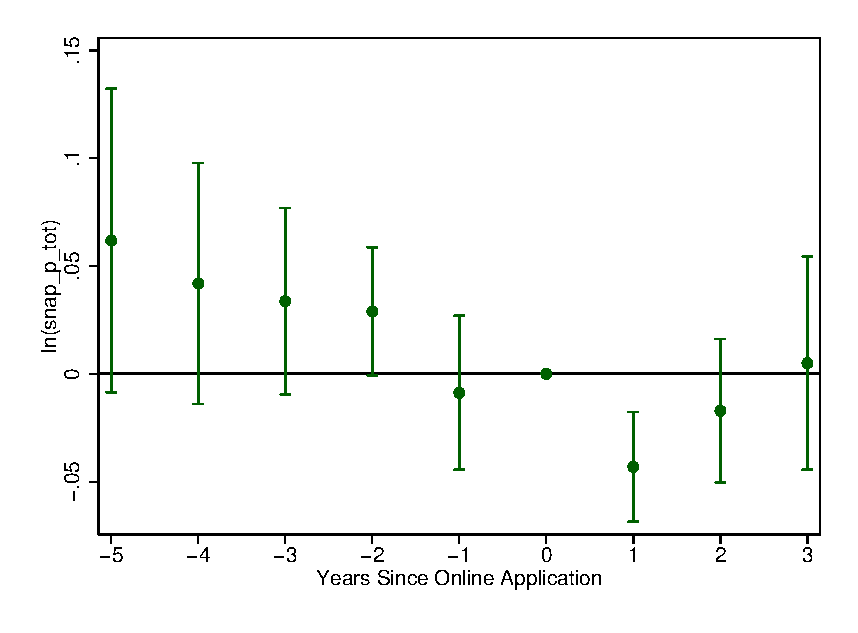
\includegraphics[scale=0.57]{tabfig/evstu_snap_p_tot_total_pop_yrcfcttru_5_3}\\
c) Year FE, County FE+Trends, UI control& c) Year FE, County FE + Trends, UI control, weighted\\
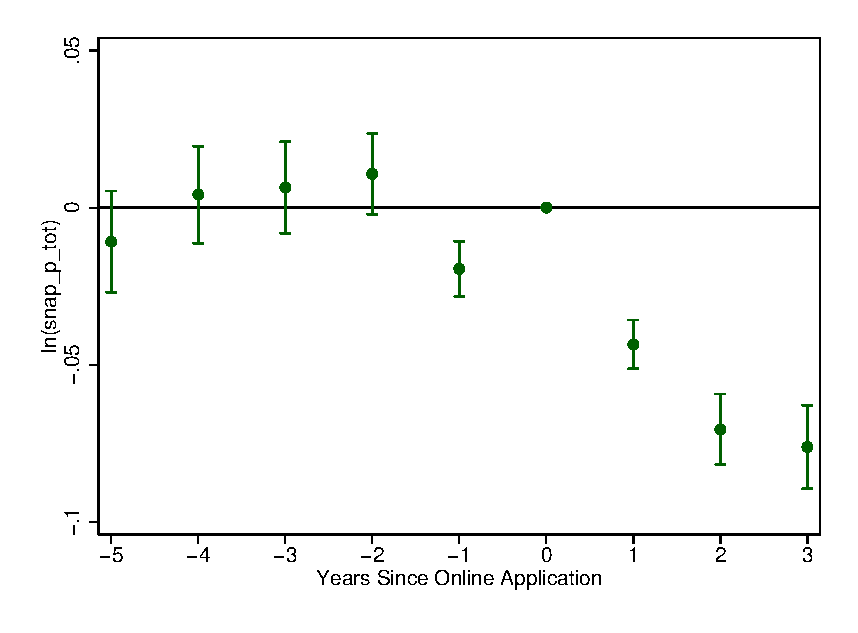
\includegraphics[scale=0.57]{tabfig/evstu_snap_p_tot_one_yrcfcttrunor_5_3}\\
e) Year FE, County FE + Trends, UI control, no Recession\\
\end{tabular}
\end{figure}

\begin{figure}\caption{Event Study Estimates, Benefits}
\begin{tabular}{cc}
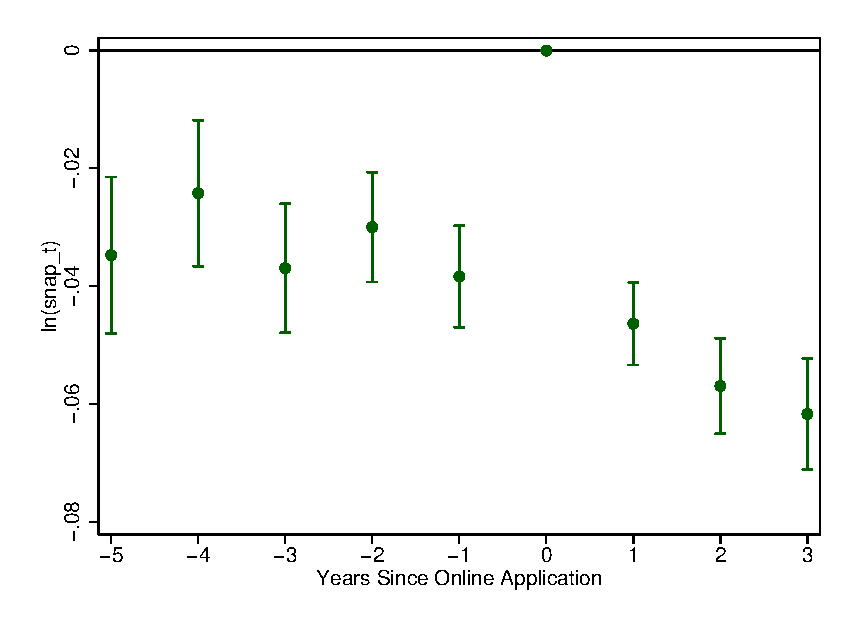
\includegraphics[scale=0.57]{tabfig/evstu_snap_t_one_yrcf_5_3}&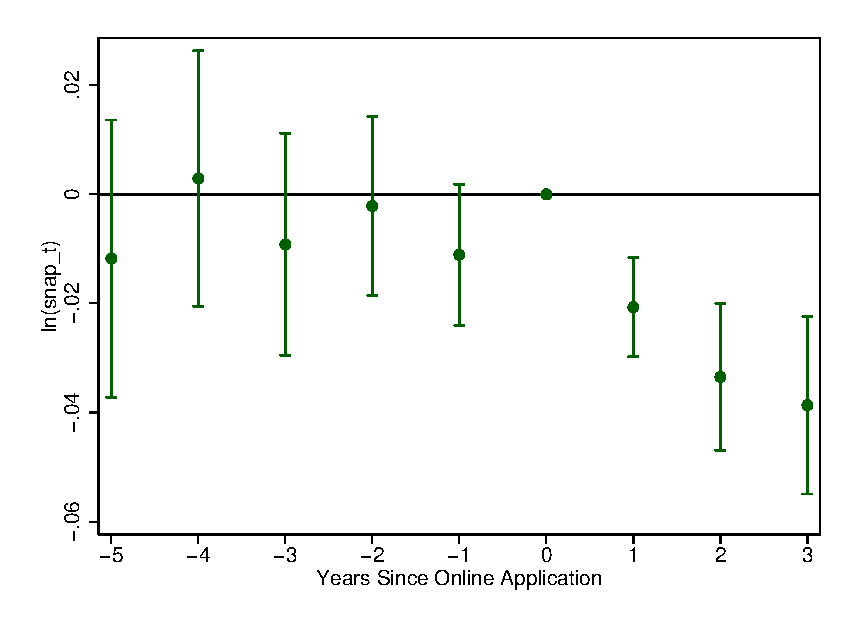
\includegraphics[scale=0.57]{tabfig/evstu_snap_t_one_yrcfsttr_5_3}\\
a) Year FE and County FE&b) Year FE, County FE+Trends\\
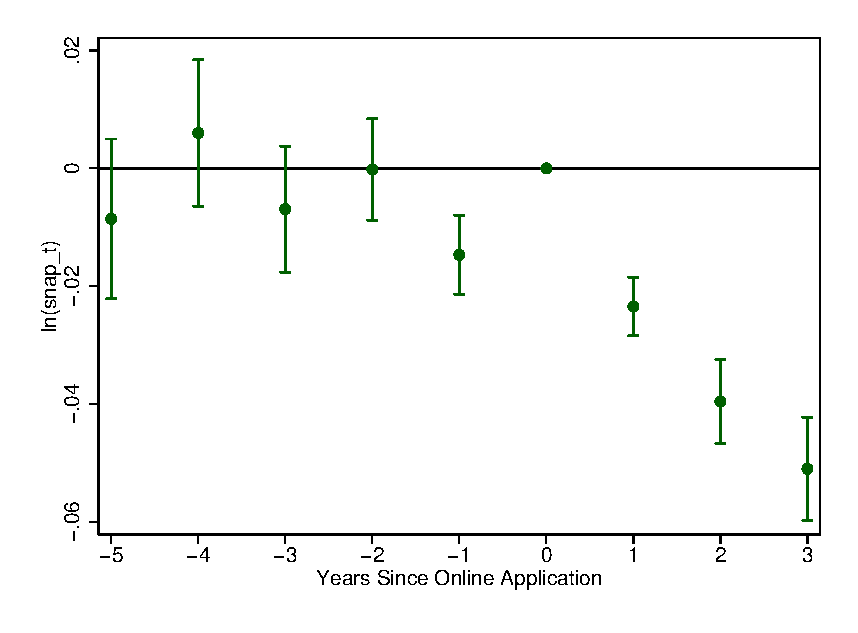
\includegraphics[scale=0.57]{tabfig/evstu_snap_t_one_yrcfcttru_5_3}&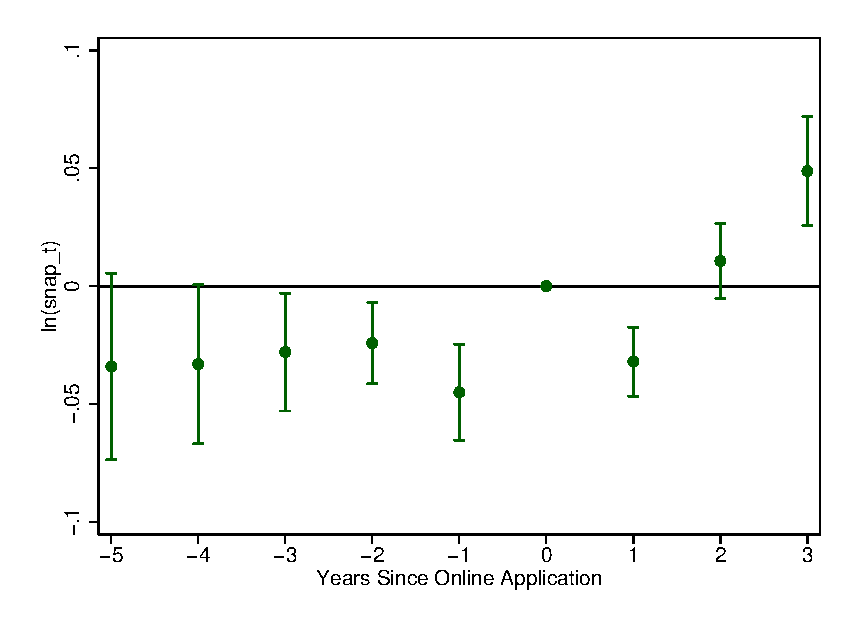
\includegraphics[scale=0.57]{tabfig/evstu_snap_t_total_pop_yrcfcttru_5_3}\\
c) Year FE, County FE+Trends, UI control& c) Year FE, County FE + Trends, UI control, weighted\\
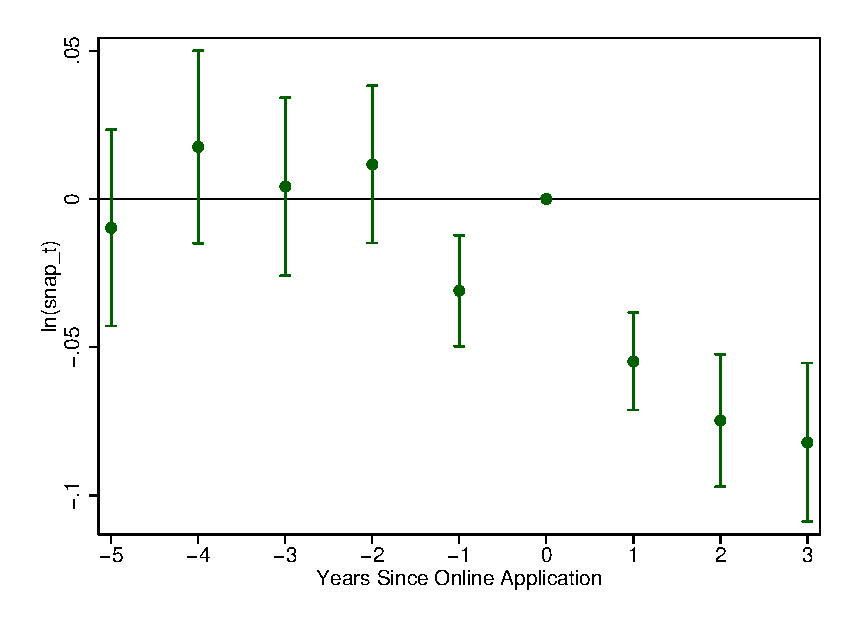
\includegraphics[scale=0.57]{tabfig/evstu_snap_t_one_yrcfcttrunor_5_3}\\
e) Year FE, County FE + Trends, UI control, no Recession\\
\end{tabular}
\end{figure}





%Population quartiles, unweighted
\begin{figure}\caption{Event Study Estimates, BEA, by County Size}
\begin{tabular}{cc}
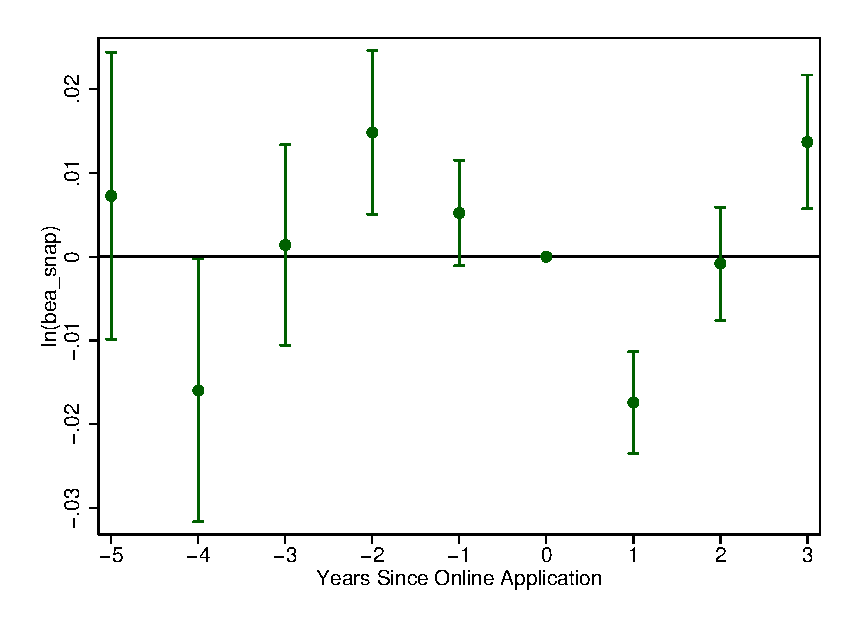
\includegraphics[scale=0.57]{tabfig/evstu_size1_bea_snap_one_yrcfcttr_5_3}&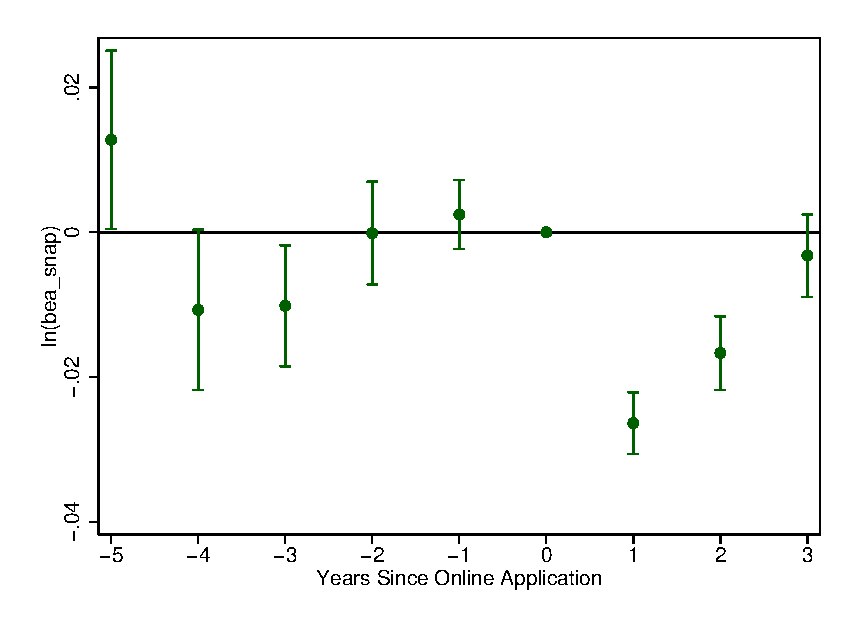
\includegraphics[scale=0.57]{tabfig/evstu_size2_bea_snap_one_yrcfcttr_5_3}\\
a) 1st Quartile&b) 2nd Quartile\\
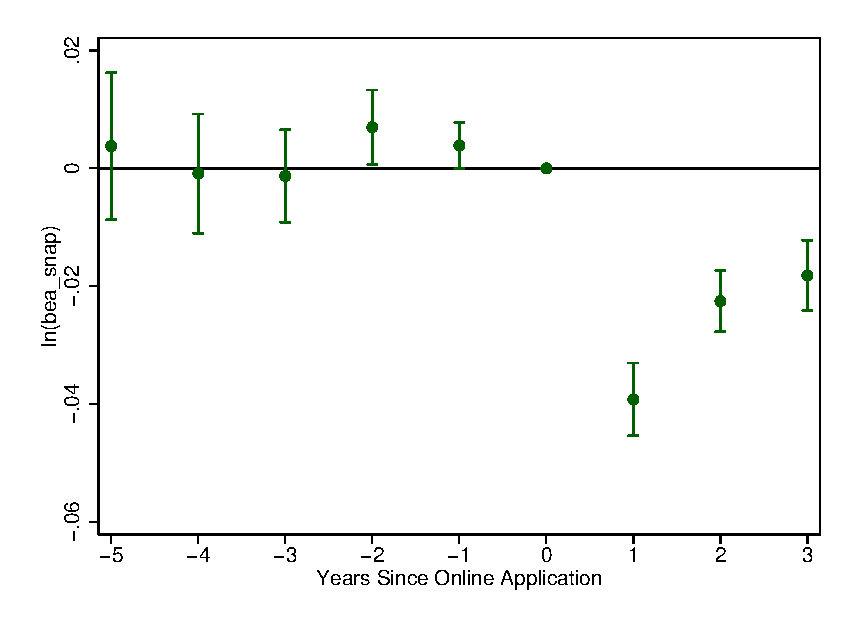
\includegraphics[scale=0.57]{tabfig/evstu_size3_bea_snap_one_yrcfcttr_5_3}&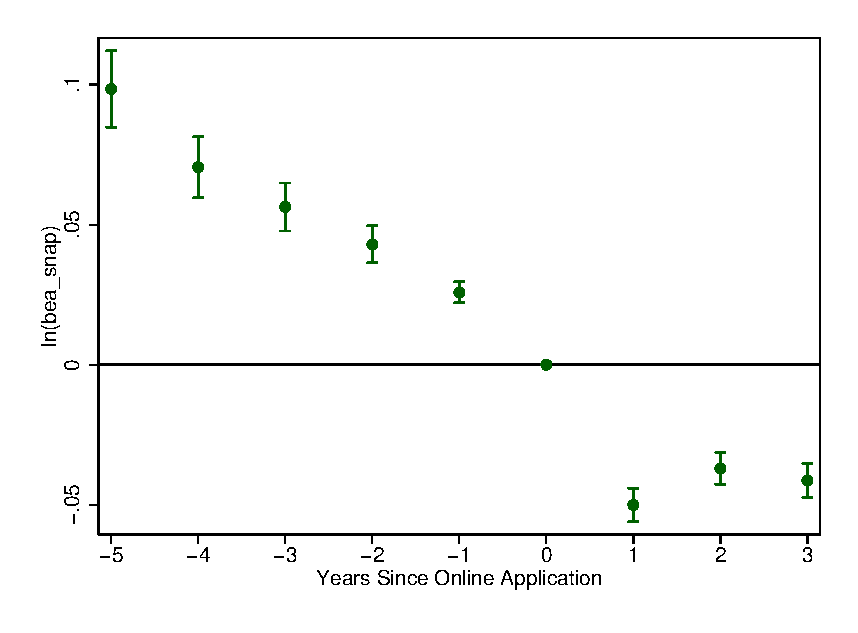
\includegraphics[scale=0.57]{tabfig/evstu_size4_bea_snap_one_yrcfcttr_5_3}\\
c) 3rd Quartile & d) 4th Quartile\\
\end{tabular}
\end{figure}


\begin{figure}\caption{Event Study Estimates, Households, by County Size}
\begin{tabular}{cc}
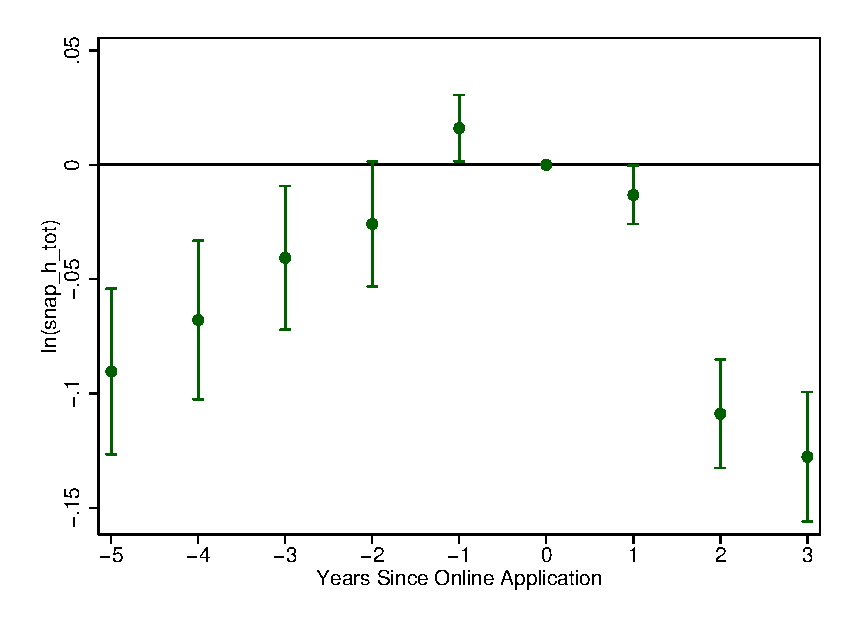
\includegraphics[scale=0.57]{tabfig/evstu_size1_snap_h_tot_one_yrcfcttr_5_3}&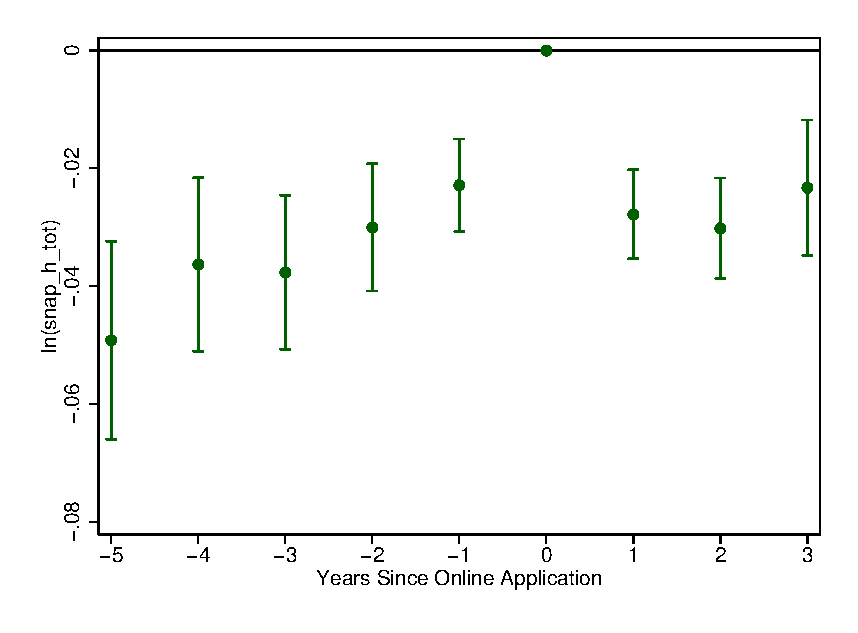
\includegraphics[scale=0.57]{tabfig/evstu_size2_snap_h_tot_one_yrcfcttr_5_3}\\
a) 1st Quartile&b) 2nd Quartile\\
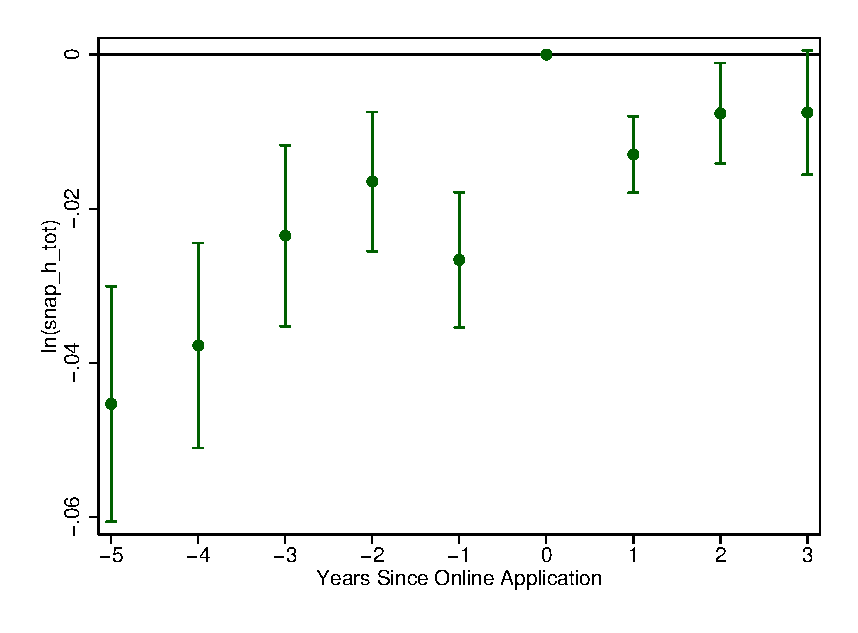
\includegraphics[scale=0.57]{tabfig/evstu_size3_snap_h_tot_one_yrcfcttr_5_3}&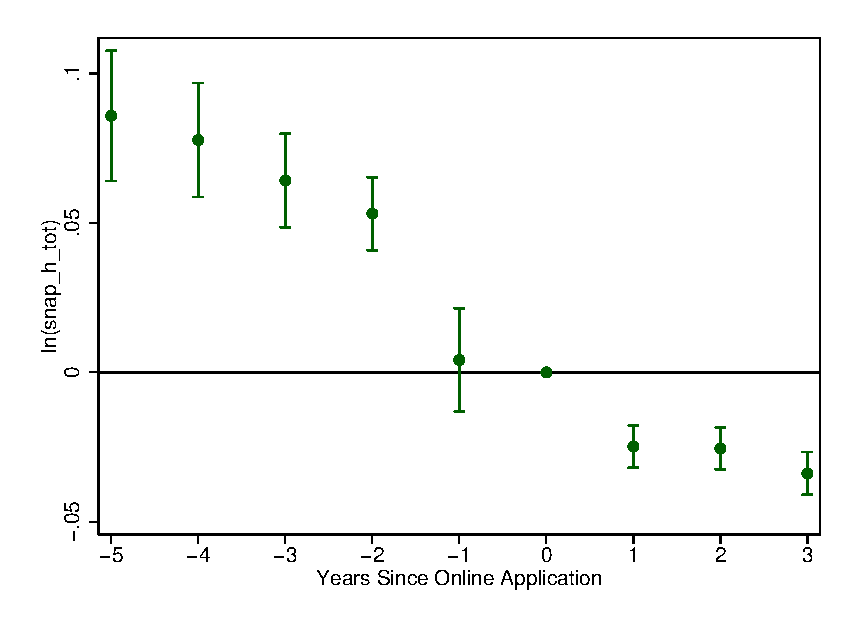
\includegraphics[scale=0.57]{tabfig/evstu_size4_snap_h_tot_one_yrcfcttr_5_3}\\
c) 3rd Quartile & d) 4th Quartile\\
\end{tabular}
\end{figure}


\begin{figure}\caption{Event Study Estimates, Individuals, by County Size}
\begin{tabular}{cc}
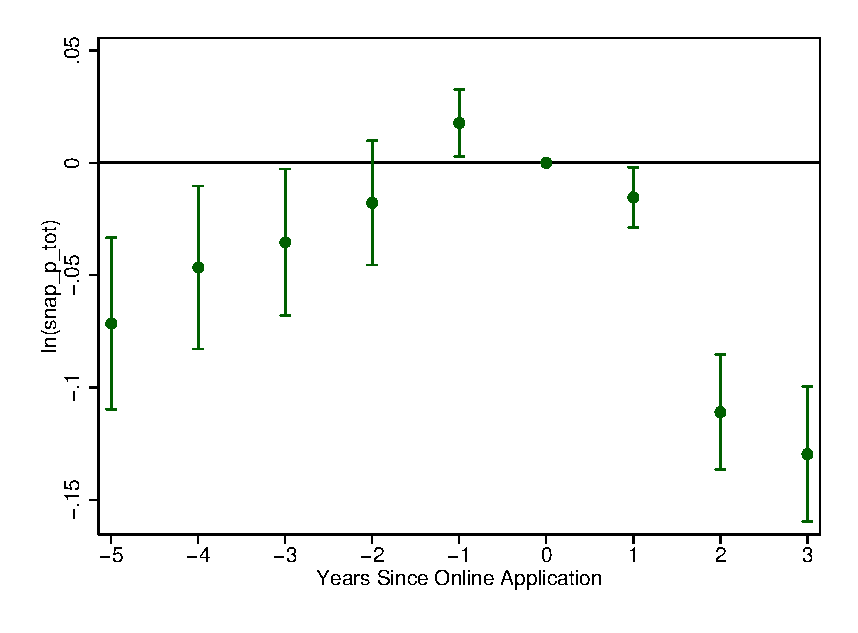
\includegraphics[scale=0.57]{tabfig/evstu_size1_snap_p_tot_one_yrcfcttr_5_3}&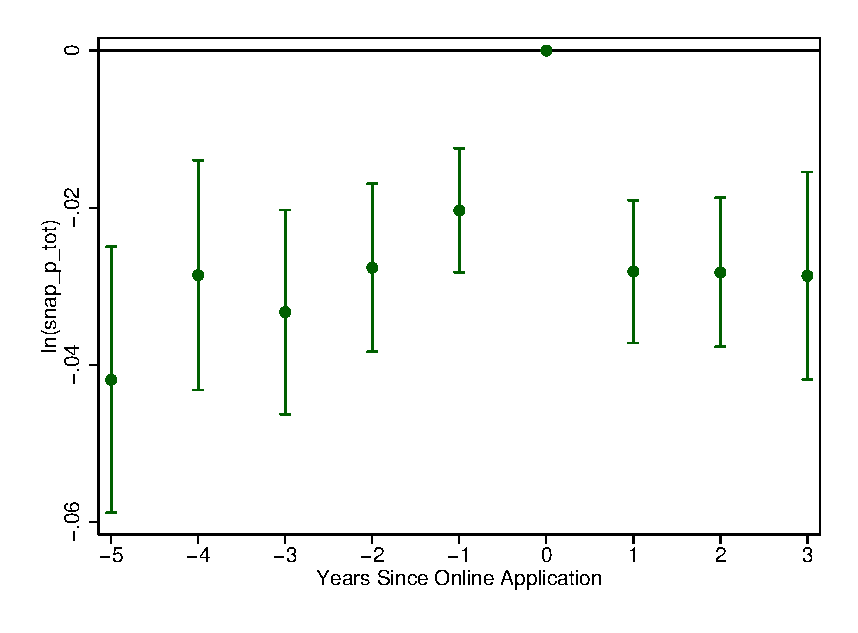
\includegraphics[scale=0.57]{tabfig/evstu_size2_snap_p_tot_one_yrcfcttr_5_3}\\
a) 1st Quartile&b) 2nd Quartile\\
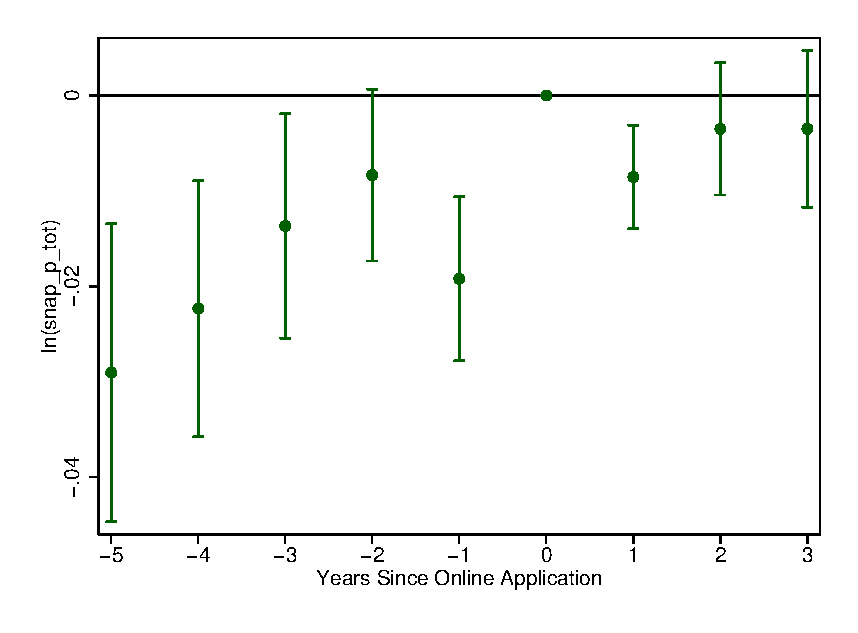
\includegraphics[scale=0.57]{tabfig/evstu_size3_snap_p_tot_one_yrcfcttr_5_3}&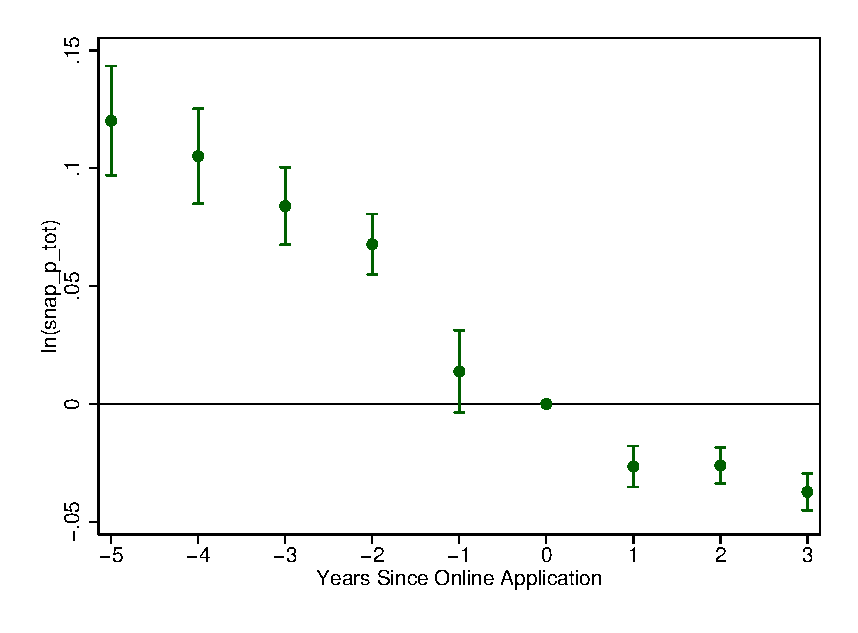
\includegraphics[scale=0.57]{tabfig/evstu_size4_snap_p_tot_one_yrcfcttr_5_3}\\
c) 3rd Quartile & d) 4th Quartile\\
\end{tabular}
\end{figure}


\begin{figure}\caption{Event Study Estimates, Benefits, by County Size}
\begin{tabular}{cc}
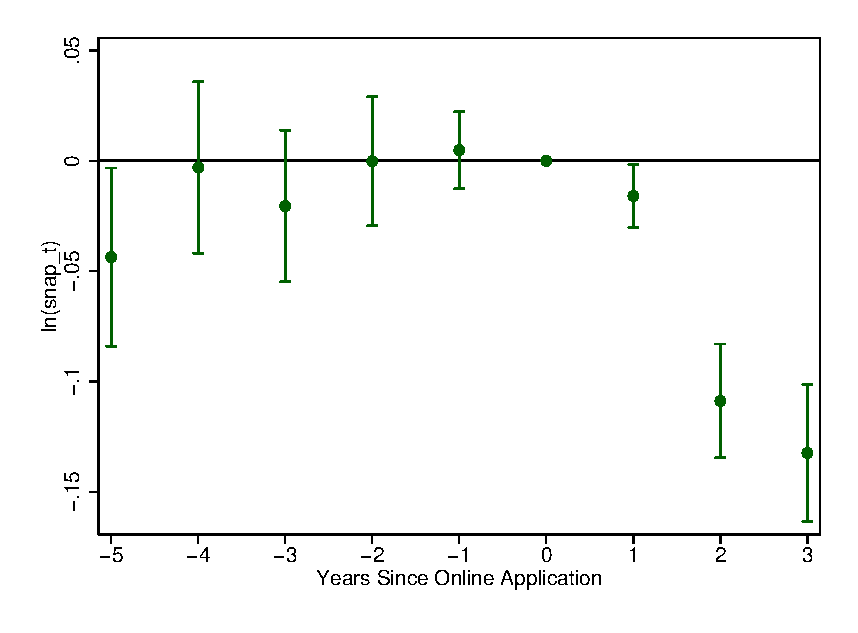
\includegraphics[scale=0.57]{tabfig/evstu_size1_snap_t_one_yrcfcttr_5_3}&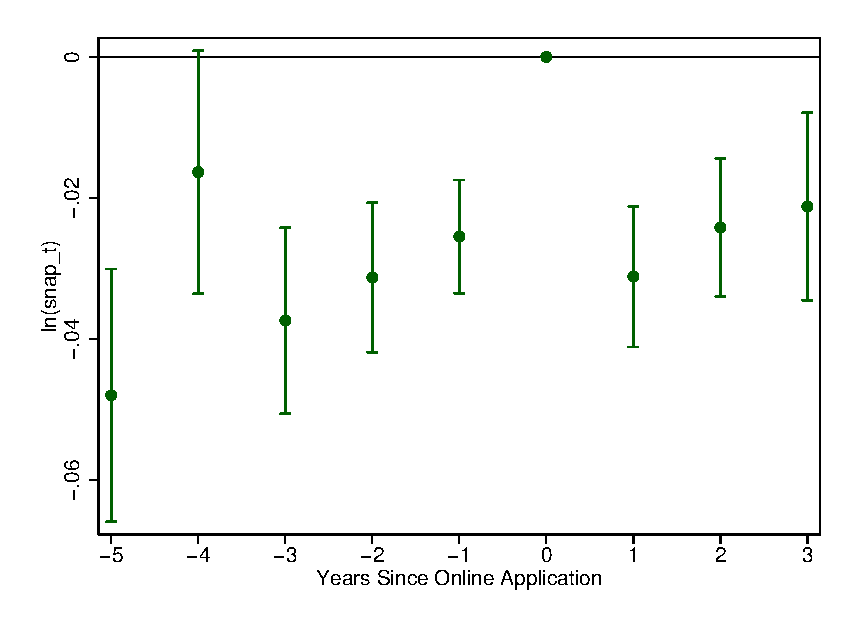
\includegraphics[scale=0.57]{tabfig/evstu_size2_snap_t_one_yrcfcttr_5_3}\\
a) 1st Quartile&b) 2nd Quartile\\
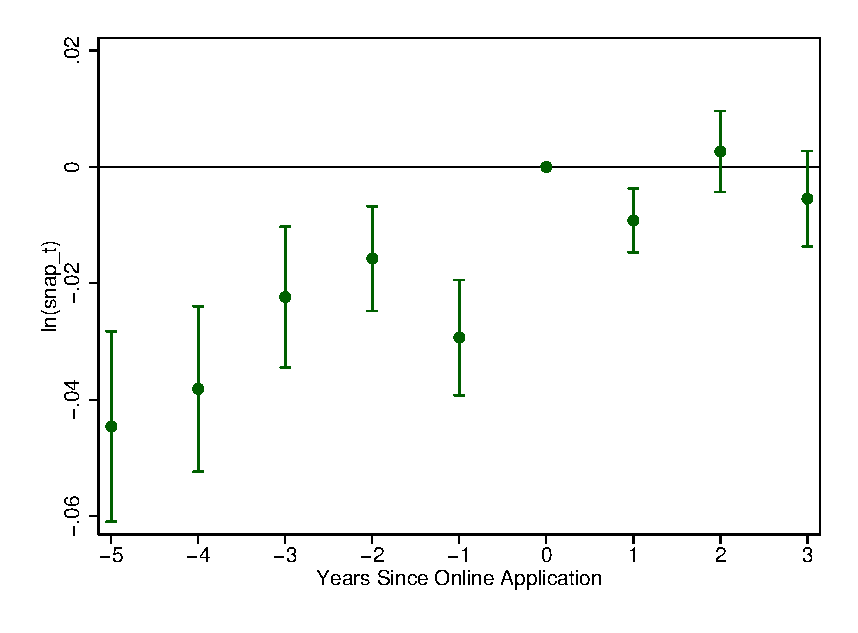
\includegraphics[scale=0.57]{tabfig/evstu_size3_snap_t_one_yrcfcttr_5_3}&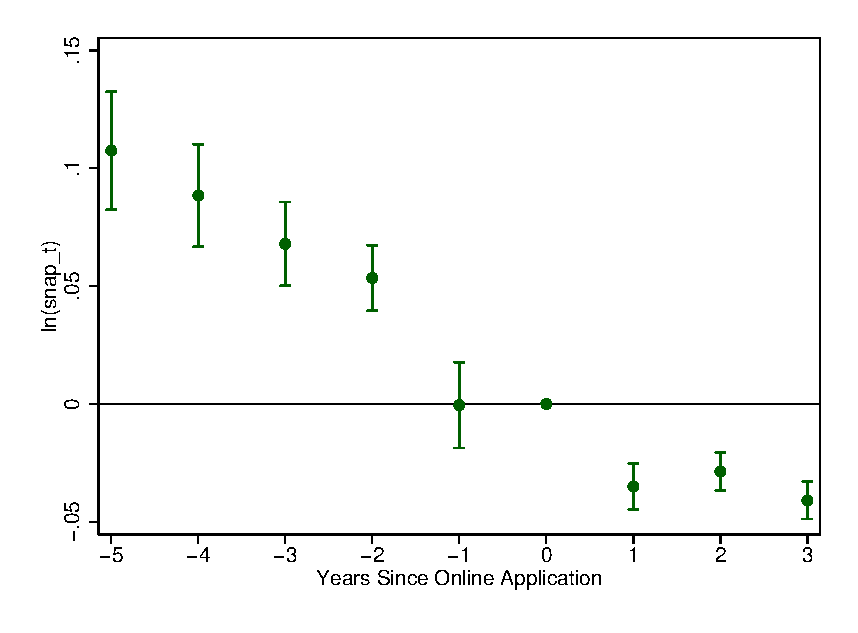
\includegraphics[scale=0.57]{tabfig/evstu_size4_snap_t_one_yrcfcttr_5_3}\\
c) 3rd Quartile & d) 4th Quartile\\
\end{tabular}
\end{figure}





\end{document}
